\section{Pipeline Template}\label{sec:template}
Our approach integrates data protection and data management into the service pipeline using annotations.
To this aim, we extend the service pipeline in \cref{def:pipeline} with: \emph{i)} data protection annotations expressing transformations on data to enforce data protection requirements, \emph{ii)} functional annotations expressing data manipulations carried out during services execution.
These annotations permit to implement an advanced data lineage, tracking the entire data lifecycle by monitoring changes arising from functional service execution and data protection requirements.

In the following, we first introduce the annotated service pipeline, called pipeline template in Section \ref{sec:templatedefinition}. We then present functional annotations (Section \ref{sec:funcannotation}) and data protection annotations (Section \ref{sec:nonfuncannotation}). We finally provide an example of a pipeline template (Section \ref{sec:example}).


\subsection{Pipeline Template Definition}\label{sec:templatedefinition}
Given the service pipeline in Definition~\ref{def:pipeline}, we use annotations to express data protection requirements to be enforced on data and functional requirements on services to be integrated in the pipeline. Each service vertex in the service pipeline is labeled with two mapping functions forming a pipeline template:
\begin{enumerate*}[label=\roman*)]
  \item a labeling function \myLambda:$\V_S\rightarrow$\P{} that associates a set of data protection requirements, in the form of policies $p$$\in$\P{}, with each vertex \vi{i}$\in$$\V_S$;
  \item a labeling function \myGamma:$\V_S\rightarrow$\F{} that associates a functional service description $F_i\in\F{}$ with each vertex \vi{i}$\in$$\V_S$.
\end{enumerate*}
%The policies will be intended to guide the enforcement of data protection while the data transformation function will characterize the functional aspect of each vertex.

The template is formally defined as follows.

\begin{definition}[Pipeline Template] \label{def:template}
  Given a service pipeline G(\V,\E), a pipeline template $G^{\myLambda,\myGamma}$(V,E,\myLambda,\myGamma) is a direct acyclic graph with two labeling functions:
  \begin{enumerate}[label=\roman*)]
    \item \myLambda that assigns a label \myLambda(\vi{i}), corresponding to a set \P{i} of policies $p_j$ to be satisfied by service $s_i$ represented by \vi{i}, for each vertex $\vi{i}\in\V_S$;
    \item \myGamma that assigns a label \myGamma(\vi{i}), corresponding to the functional description $F_i$ of service $s_i$ represented by \vi{i}, for each vertex $\vi{i}\in\V_S$.
  \end{enumerate}
\end{definition}

We note that, at this stage, the template is not yet linked to any services, nor it is possible to determine the policy modeling the specific data protection requirements.
We also note that policies $p_j$$\in$\P{i} annotated with \myLambda(\vi{i}) are ORed, meaning that the access decision is positive if at least one policy $p_j$ is evaluated to \emph{true}.
      %We also note that functional description $F_i$ includes the specific data transformation triggered as the result of a service execution.
      An example of pipeline template is depicted in \cref{fig:service_composition_template}

      %The next sections better explain the functional and non-functional transformation functions.
      \begin{figure}[ht!]
        \centering
        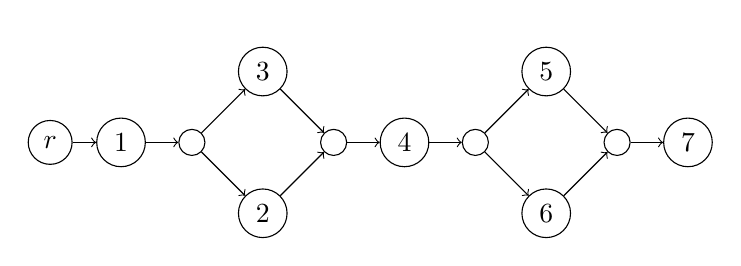
\begin{tikzpicture}[scale=0.9]
          % Nodes
          \node[draw, circle] (node1) at (0,0) {$\s{r}$};
          \node[draw, circle] (node2) at (1,0) {$\s{1}$};
          \node[draw, circle] (node3) at (2,0) {$\timesOperator$};
          \node[draw, circle] (node4) at (3,-1) {$\s{2}$};
          \node[draw, circle] (node5) at (3,1) {$\s{3}$};
          \node[draw, circle] (node6) at (4,0) {$\timesOperator$};
          \node[draw, circle] (node65) at (5,0) {$\s{4}$};
          \node[draw, circle] (node7) at (6,0) {$\plusOperator$};
          \node[draw, circle] (node8) at (7,1) {$\s{5}$};
          \node[draw, circle] (node9) at (7,-1) {$\s{6}$};
          \node[draw, circle] (node10) at (8,0) {$\plusOperator$};
          \node[draw, circle] (node11) at (9,0) {$\s{7}$};
          % Text on top
          \node[above] at (node1.north)  {$\templateChartAnnotation$};
          \node[above] at (node2.north)  {$\templateChartAnnotation$};
          \node[above] at (node3.north)  {                 };
          \node[above] at (node4.north)  {$\templateChartAnnotation$};
          \node[above] at (node5.north)  {$\templateChartAnnotation$};
          \node[above] at (node65.north) {$\templateChartAnnotation$};
          \node[above] at (node8.north)  {$\templateChartAnnotation$};
          \node[above] at (node9.north)  {$\templateChartAnnotation$};
          \node[above] at (node11.north) {$\templateChartAnnotation$};
          % Connection
          \draw[->] (node1) -- (node2);
          \draw[->] (node2) -- (node3);
          \draw[->] (node3) -- (node4);
          \draw[->] (node3) -- (node5);
          \draw[->] (node5) -- (node6);
          \draw[->] (node4) -- (node6);
          \draw[->] (node6) -- (node65);
          \draw[->] (node65) -- (node7);
          \draw[->] (node7) -- (node8);
          \draw[->] (node7) -- (node9);
          \draw[->] (node8) -- (node10);
          \draw[->] (node9) -- (node10);
          \draw[->] (node10) -- (node11);
        \end{tikzpicture}
        \caption{Pipeline Template}
        \label{fig:service_composition_template}
      \end{figure}




      % \begin{figure}[ht!]
      %   \centering
      %   \begin{tikzpicture}
      %     % Nodes
      %     \node[draw, circle,minimum size=1cm] (node1) at (0,0) {$\s{1}$};
      %     \node[draw, circle,minimum size=1cm] (node2) at (2,0) {$\s{2}$};
      %     \node[draw, circle,minimum size=1cm] (node3) at (4,0) {$\s{3}$};

      %     \node[above] at (node1.north)  {$\templateChartAnnotation$};
      %     \node[above] at (node2.north)  {$\templateChartAnnotation$};
      %     \node[above] at (node3.north)  {$\templateChartAnnotation$};

      %     % Connection
      %     \draw[->] (node1) -- (node2);
      %     \draw[->] (node2) -- (node3);

      %   \end{tikzpicture}
      %   \caption{Pipeline Template Example}
      %   \label{fig:temp}
      % \end{figure}

      \subsection{Data Protection Annotation}\label{sec:nonfuncannotation}
      Data Protection Annotation \myLambda\ expresses data protection requirements in the form of access control policies. We consider an attribute-based access control model that offers flexible fine-grained authorization and adapts its standard key components to address the unique characteristics of a big data environment. Access requirements are expressed in the form of policy conditions that are defined as follows.

      \begin{definition}[Policy Condition]\label{def:policy_cond}
        A \emph{Policy Condition pc} is a Boolean expression of the form $($\emph{attr\_name} op \emph{attr\_value}$)$, with op$\in$\{$<$,$>$,$=$,$\neq$,$\leq$,$\geq$\}, \emph{attr\_name} an attribute label, and \emph{attr\_value} the corresponding attribute value.
      \end{definition}

      An access control policy then specifies who (\emph{subject}) can access what (\emph{object}) with action (\emph{action}), in a specific context (\emph{environment}) and under specific obligations (\emph{data transformation}), as formally defined below.

      \begin{definition}[Policy]\label{def:policy_rule}
        A {\it policy p}$\in$\P{} is 5-uple $<$\textit{subj}, \textit{obj}, \textit{act}, \textit{env}, \textit{\TP}$>$, where:
        \begin{description}
          \item Subject \textit{subj} defines a service $s_i$ issuing an access request to perform an action on an object. It is of the form $<$\emph{id}, \{$pc_i$\}$>$, where \emph{id} defines a class of services (e.g., classifier), and \{$pc_i$\} is a set of \emph{Policy Conditions} on the subject, as defined in Definition \ref{def:policy_cond}. For instance, $<$\emph{service},\{(classifier $=$ "SVM")\}$>$ refers to a service providing a SVM classifier. We note that \textit{subj} can also specify conditions on the service owner, such as, $<$\emph{service},\{(owner\_location $=$ "EU")\}$>$ and on the service user, such as, $<$\emph{service},\{(service\_user\_role $=$ "DOC Director")\}$>$.

          \item Object \textit{obj} defines any data whose access is governed by the policy. It is of the form $<$\emph{type}, \{$pc_i$\}$>$, where: \emph{type} defines the type of object, such as a file (e.g., a video, text file, image, etc.), a SQL or noSQL database, a table, a column, a row, or a cell of a table, and \{$pc_i$\} is a set of \emph{Policy Conditions} defined on the object's attributes. For instance, $<$\emph{dataset},\{(region $=$ CT)\}$>$ refers to a dataset whose region is Connecticut.

          \item Action \textit{act} defines any operations that can be performed within a big data environment, from traditional atomic operations on databases (e.g., CRUD operations varying depending on the data model) to coarser operations, such as an Apache Spark Direct Acyclic Graph (DAG), Hadoop MapReduce, an analytics function call, or an analytics pipeline.

          \item Environment \textit{env} defines a set of conditions on contextual attributes, such as time of the day, location, IP address, risk level, weather condition, holiday/workday, emergency. It is a set \{$pc_i$\} of \emph{Policy Conditions} as defined in Definition \ref{def:policy_cond}. For instance, $<$\emph{env},\{(time $=$ "night")\}$>$ refers to a policy that is applicable only at night.

          \item Data Transformation \textit{\TP} defines a set of security and privacy-aware transformations on \textit{obj}, which must be enforced before any access to data.
                Transformations focus on data protection, as well as compliance to regulations and standards, in addition to simple format conversions.
                For instance, let us define three transformations that can be applied to the \cref{tab:dataset}:     \begin{enumerate*}[label=\roman*)]
                  \item \emph{level0} (\tp{0}): no anonymization is carried out;
                        The data has been partially anonymized with only the first name and last name being anonymized.
                  \item \emph{level1} (\tp{2}): \item \emph{level2} (\tp{2}): The data has been fully anonymized with the first name, last name, identifier, and age being anonymized.
                \end{enumerate*}
        \end{description}
      \end{definition}

      Access control policies $p_j$$\in$\P{i} annotating vertex \vi{i} in a pipeline template $G^{\myLambda,\myGamma}$ are used to filter out those candidate services $s$$\in$$S^c$ that do not match data protection requirements. Specifically, each policy $p_j$$\in$\P{i} is evaluated to verify whether a candidate service $s$$\in$$S^c$ for vertex \vi{i} is compatible with data protection requirements in \P{i} (\myLambda(\vi{i})). Policy evaluation matches the profile of candidate service $s$$\in$$S^c$ with the policy conditions in each $p_j$$\in$\P{i}. If the credentials and attributes in the candidate service profile fails to meet the policy conditions, meaning that no policies $p_j$ are evaluated to \emph{true}, the service is discarded; otherwise it is added to the set $S'$ of compatible service, which is used in Section~\ref{sec:instance} to generate the pipeline instance $G'$. No policy enforcement is done at this stage.
    \subsection{Functional Annotations}\label{sec:funcannotation}
    A proper data management approach must track functional data manipulations across the entire pipeline execution, defining the functional requirements of each service operating on data.
    To this aim, each vertex \vi{i}$\in\V_S$ is annotated with a label \myGamma(\vi{i}), corresponding to the functional description $F_i$ of the service $s_i$ represented by \vi{i}.
  $F_i$ describes the functional requirements on the corresponding service $s_i$, such as API, inputs, expected outputs.
    %The latter is modeled as a functional transformation function \TF\ that is applied to the data when executing service $s_i$. \TF\ has a twofold role:
    %\begin{enumerate}[label=\roman*)]
    %  \item it contains the functional requirements that the service must satisfy, in terms of expected input, expected output, prototype and other functional aspects.
    %  \item
    It also specifies a set \TF{} of data transformation functions \tf{i}, possibly triggered during execution of the connected service $s_i$.

    Each $\tf{i}$$\in$$\TF{}$ can be of different types as follows:
\begin{enumerate*}[label=\roman*)]
  \item an empty function \tf{\epsilon} that applies no transformation or processing on the data;
  \item an additive function \tf{a} that expands the amount of data received, for example, by integrating data from other sources;
  \item a transformation function \tf{t} that transforms some records in the dataset without altering the domain;
  \item a transformation function \tf{d} (out of the scope of this work) that changes the domain of the data by applying, for instance, PCA or K-means.
\end{enumerate*}

For simplicity but with no loss of generality, we assume that all candidate services meet functional annotation \F{} and that \TF{}=\tf{}. As a consequence, all candidate services apply the same transformation to data during execution.

